\documentclass[tikz,border=10pt]{standalone}
% Scale s = 0.021277 cm/px, origin from ink-bbox centre (226, 208.5) px
\begin{document}
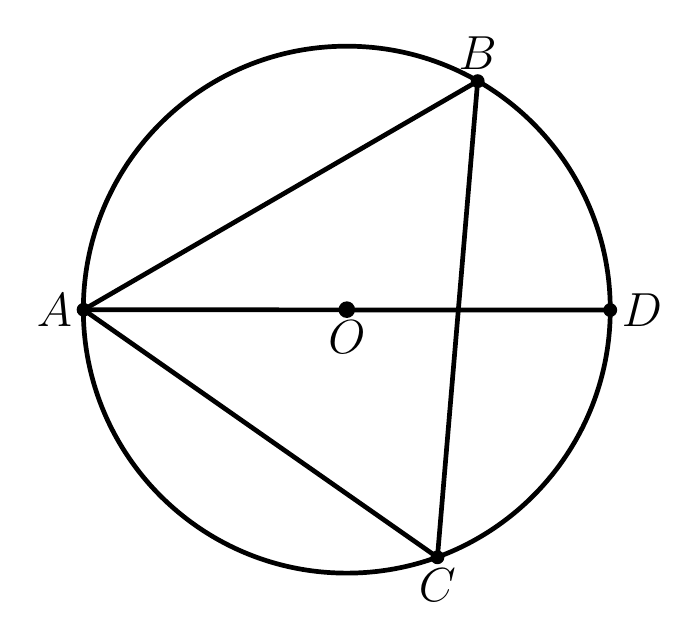
\begin{tikzpicture}[line width=1.7pt, line join=round]

% Named coordinates (converted from pixels)
\coordinate (O) at (-0.037,0.143);
\coordinate (A) at (-3.380,0.142);
\coordinate (D) at (3.309,0.138);
\coordinate (B) at (1.625,3.045);
\coordinate (C) at (1.114,-3.002);

% Circle: centre O, radius 157.27 px = 3.346 cm
\draw (O) circle[radius=3.346];

% Diameter AD
\draw (A) -- (D);

% Chords
\draw (A) -- (B);
\draw (A) -- (C);
\draw (B) -- (C);

% Point markers (drawn after the lines so they sit on top); enlarged dots
\fill[black] (A) circle (2.5pt);
\fill[black] (B) circle (2.5pt);
\fill[black] (C) circle (2.5pt);
\fill[black] (D) circle (2.5pt);
\fill[black] (O) circle (3pt);

% Labels (font from style metrics)
\node[left,  font=\fontsize{17.5}{21}\selectfont] at (A) {$A$};
\node[right, font=\fontsize{17.5}{21}\selectfont] at (D) {$D$};
\node[above, font=\fontsize{17.5}{21}\selectfont] at (B) {$B$};
\node[below, font=\fontsize{17.5}{21}\selectfont] at (C) {$C$};
\node[below, font=\fontsize{17.5}{21}\selectfont] at (O) {$O$};

\end{tikzpicture}
\end{document}